\documentclass[border=6pt]{standalone}
\usepackage{tikz}
\usepackage[edges]{forest}
\usetikzlibrary{arrows.meta,positioning,calc,decorations.pathreplacing,shapes.geometric}
\begin{document}
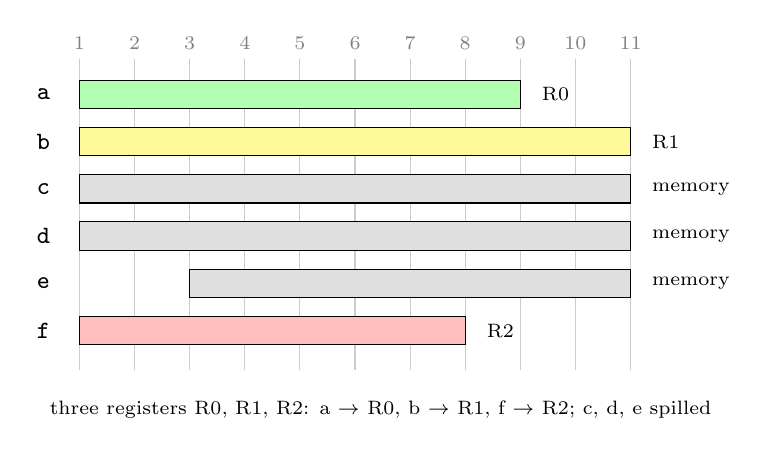
\begin{tikzpicture}[font=\small]
\node[font=\scriptsize,gray] at (0.70,0.45) {1};
\draw[gray!40] (0.70,0.25) -- (0.70,-3.70);
\node[font=\scriptsize,gray] at (1.40,0.45) {2};
\draw[gray!40] (1.40,0.25) -- (1.40,-3.70);
\node[font=\scriptsize,gray] at (2.10,0.45) {3};
\draw[gray!40] (2.10,0.25) -- (2.10,-3.70);
\node[font=\scriptsize,gray] at (2.80,0.45) {4};
\draw[gray!40] (2.80,0.25) -- (2.80,-3.70);
\node[font=\scriptsize,gray] at (3.50,0.45) {5};
\draw[gray!40] (3.50,0.25) -- (3.50,-3.70);
\node[font=\scriptsize,gray] at (4.20,0.45) {6};
\draw[gray!40] (4.20,0.25) -- (4.20,-3.70);
\node[font=\scriptsize,gray] at (4.90,0.45) {7};
\draw[gray!40] (4.90,0.25) -- (4.90,-3.70);
\node[font=\scriptsize,gray] at (5.60,0.45) {8};
\draw[gray!40] (5.60,0.25) -- (5.60,-3.70);
\node[font=\scriptsize,gray] at (6.30,0.45) {9};
\draw[gray!40] (6.30,0.25) -- (6.30,-3.70);
\node[font=\scriptsize,gray] at (7.00,0.45) {10};
\draw[gray!40] (7.00,0.25) -- (7.00,-3.70);
\node[font=\scriptsize,gray] at (7.70,0.45) {11};
\draw[gray!40] (7.70,0.25) -- (7.70,-3.70);
\node[anchor=east] at (0.45,-0.20) {\texttt{a}};
\fill[green!30,draw=black] (0.70,-0.38) rectangle (6.30,-0.02);
\node[font=\scriptsize,anchor=west] at (6.45,-0.20) {R0};
\node[anchor=east] at (0.45,-0.80) {\texttt{b}};
\fill[yellow!40,draw=black] (0.70,-0.98) rectangle (7.70,-0.62);
\node[font=\scriptsize,anchor=west] at (7.85,-0.80) {R1};
\node[anchor=east] at (0.45,-1.40) {\texttt{c}};
\fill[gray!25,draw=black] (0.70,-1.58) rectangle (7.70,-1.22);
\node[font=\scriptsize,anchor=west] at (7.85,-1.40) {memory};
\node[anchor=east] at (0.45,-2.00) {\texttt{d}};
\fill[gray!25,draw=black] (0.70,-2.18) rectangle (7.70,-1.82);
\node[font=\scriptsize,anchor=west] at (7.85,-2.00) {memory};
\node[anchor=east] at (0.45,-2.60) {\texttt{e}};
\fill[gray!25,draw=black] (2.10,-2.78) rectangle (7.70,-2.42);
\node[font=\scriptsize,anchor=west] at (7.85,-2.60) {memory};
\node[anchor=east] at (0.45,-3.20) {\texttt{f}};
\fill[red!25,draw=black] (0.70,-3.38) rectangle (5.60,-3.02);
\node[font=\scriptsize,anchor=west] at (5.75,-3.20) {R2};
\node[font=\scriptsize,anchor=west] at (0.2,-4.2) {three registers R0, R1, R2: a $\to$ R0, b $\to$ R1, f $\to$ R2; c, d, e spilled};
\end{tikzpicture}
\end{document}
